\documentclass{report}
\usepackage[utf8]{inputenc}
\usepackage[francais]{babel}
\usepackage[T1]{fontenc}
\usepackage{lmodern}
\usepackage{textcomp}
\usepackage{listings}
\usepackage{graphicx}
\usepackage{hyperref}
\usepackage{titlesec}
\usepackage{tcolorbox}
\usepackage{amsmath}
\usepackage{color}
\usepackage{multirow}
\setcounter{tocdepth}{5}
\setcounter{secnumdepth}{4}
\definecolor{dkgreen}{rgb}{0,0.6,0}
\definecolor{gray}{rgb}{0.5,0.5,0.5}
\definecolor{mauve}{rgb}{0.58,0,0.82}
\definecolor{gray}{rgb}{0.4,0.4,0.4}
\definecolor{darkblue}{rgb}{0.0,0.0,0.6}
\titleformat{\paragraph}
{\normalfont\normalsize\bfseries}{\theparagraph}{1em}{}
\titlespacing*{\paragraph}
{0pt}{3.25ex plus 1ex minus .2ex}{1.5ex plus .2ex}
\renewcommand{\thesection}{\Roman{section}}
\hypersetup{
    colorlinks=true,
    linkcolor=black,
    filecolor=magenta,
    urlcolor=cyan,
}
\lstnewenvironment{cc}
{
\lstset{frame=tblr,
  language=C,
  aboveskip=3mm,
  belowskip=3mm,
  showstringspaces=false,
  columns=flexible,
  basicstyle={\small\ttfamily},
  numbers=none,
  numberstyle=\tiny\color{gray},
  keywordstyle=\color{blue},
  commentstyle=\color{dkgreen},
  stringstyle=\color{mauve},
  breaklines=true,
  breakatwhitespace=true,
  tabsize=3
}}
{}

\begin{document}
\title{
  \begin{minipage}\linewidth
      \centering
      Projet AOA sujet 10 \textcopyleft
      \vskip 5pt
      \author{
        ALEXANDRE Julien \\
        \texttt{julien.alexandre@isty.uvsq.fr}
      \and
        VIRLOGEUX Marin \\
        \texttt{marin.virlogeux@isty.uvsq.fr}
      \and
        LEDOYEN Paul \\
        \texttt{paul.ledoyen@isty.uvsq.fr}
      \and
        DRISSI Mohamed Reda \\
        \texttt{reda-mohamed@isty.uvsq.fr}
      }
    \end{minipage}
}
\maketitle
\newpage
\tableofcontents
\newpage
\section{Introduction}
 \subsection{Objectifs}
  	L'objectif de ce projet est d'étudier un noyau de code et d'optimiser sa compilation. Nous traitons ici la phase I de ce projet qui consiste en
  	\begin{itemize}
  	\item mesurer la performance du noyau pour différents niveaux d'optimisations de GCC\textsuperscript \textcopyleft   et d'ICC
  	\item trouver d'autres options d'optimisations pertinentes
	\item expliquer les différences de performances entre versions d'optimisation avec MAQAO ou likwid
	\item justifier l'implémentation du driver
  	\end{itemize}
  \subsection{Spécifications de la machine utilisée}
  Nous avons traité les différents cas sur la même machine pour conserver une certaine constance dans les mesures effectuées.
    \begin{itemize}
      \item CPU : \href{https://ark.intel.com/products/88195/Intel-Core-i7-6700K-Processor-8M-Cache-up-to-4_20-GHz}
        {intel core i7 6700K 4.0GHZ 4 physical cores, 8 logical(HyperThreading©) turbo boost off}
      \item RAM : Corsair CMK16GX4M2B3000C15 Vengeance LPX 16GB DDR4 3000MHz C15 XMP 2.0
      \item Stockage : \href{http://downloadcenter.samsung.com/content/UM/201711/20171115103115156/Samsung_SSD_850_PRO_Data_Sheet_Rev_3.pdf}
          {Samsung 850 PRO SSD 512GB}
    \end{itemize}
    \subsection{Système}
      \begin{itemize}
      \item OS : Debian 9.4 Stretch (stable) x86\_64
      \item Kernel :  4.9.0-6-amd64
      \item GCC\textsuperscript \textcopyleft   : 6.3.0 20170516 (Debian 6.3.0-18+deb9u1)
      \item ICC : 18.0.1 20171018
    \end{itemize}
  \subsection{Topologie du système}
    \begin{figure}[ht!]
      \centering
      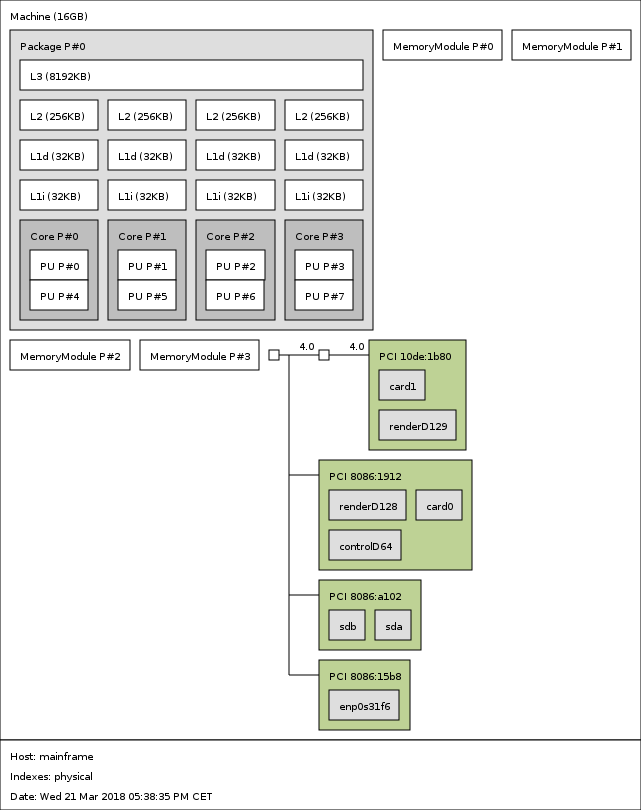
\includegraphics[scale=0.35]{resources/lstopo.png}
      \caption{Topologie générée par \href{https://manpages.debian.org/jessie/hwloc/lstopo.1.en.html}{lstopo}}
    \end{figure}
  \newpage
  \subsection{Noyau}
  Le noyau traité est le suivant :
    \lstinputlisting[language=c]{../subject10.c}

\newpage
\section{Détermination des paramètres}
  \subsection{Taille des données}
    Notre boucle utilise un tableau de \texttt{double} de taille $n\times n$
    chaque case prend 8 octets. \\
    Donc le coût total (en mémoire) de notre boucle sera de $8n^2$ . \\

    Si nous voulons utiliser L1, L2, L3 ou la ram il faut trouver l'intervalle de chacun
    Soit T la taille maximale (qui serait en puissance de 2 alors $T=2^t$) :
    \begin{align}
      8n^2 \leq 2^t \\
      n \leq 2^{\frac{t-3}{2}}
    \end{align}
    Les données des différents caches et ram sont
    \begin{itemize}
      \item L1 : 32Ko   = $2^{15}$ octets
      \item L2 : 256Ko  = $2^{18}$ octets
      \item L3 : 8192Ko = $2^{23}$ octets
      \item RAM: 16Gb   = $2^{34}$ octets
    \end{itemize}
    \vspace{5mm}
    \begin{tabular}{|l| c | c | c|}
      \hline
      Mémoire & $2^t$ & Taille & coût \\\hline
      \hline
      L1 & 15 & 64 & 31.64Ko \\\hline
      L2 & 18 & 181 & 256Ko \\\hline
      L3 & 23 & 1024 & 8190Ko \\\hline
      RAM & 34 & 46340 & 16Gb \\\hline
    \end{tabular}

   Par précaution, nous n'allons pas prendre des tailles de tableau exactement identiques aux tailles maximales des caches, pour éviter tout débordement.
    \subsection{Nombre de warmup}
    Nous allons étudier pour chaque taille de tableau, et pour chaque option d'optimisations le nombre de cycles nécessaires (ordonnée) pour chaque itération de warmup (abscisse). On pourra ainsi déterminer approximativement le nombre de warmup necessaires pour atteindre le régime permanent.
    \subsubsection{L1 : taille 60}
      \newpage
      \paragraph{compilateur \texttt{GCC\textsuperscript \textcopyleft  }}
        \subparagraph{ \texttt{Optimisation O2}}
      Nous trouvons ce résultat pour L1 :
      \begin{figure}[ht!]
        \centering
        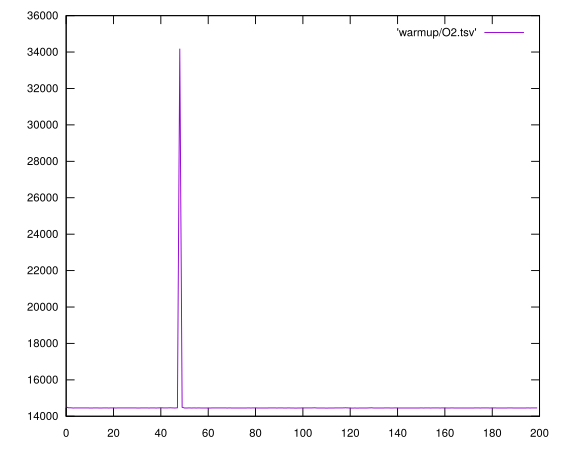
\includegraphics[scale=0.45]{resources/L1/warmup/O2.png}
        \caption{Résultat du warmup avec option \texttt{O2} du compilateur \textbf{GCC\textsuperscript \textcopyleft  }}
      \end{figure}

      Le pic observé correspond à une interférence, nous n'en tiendrons donc pas compte. On observe que le régime permanent est atteint très vite, on appliquera donc 20 warmups.
      \newpage
      \subparagraph{ \texttt{Optimisation O3}}
    Nous trouvons ce résultat pour L1 :
    \begin{figure}[ht!]
      \centering
      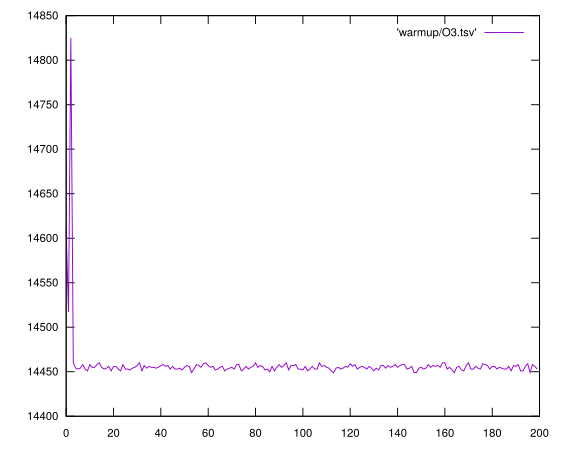
\includegraphics[scale=0.45]{resources/L1/warmup/O3.png}
      \caption{Résultat du warmup avec option \texttt{O3} du compilateur \textbf{GCC\textsuperscript \textcopyleft  }}
    \end{figure}

    Ici on observe un régime transitoire de très faible durée, un nombre de warmups de 20 est également suffisant.
    \newpage
\subparagraph{ \texttt{Optimisation O3 march=native}}
  Nous trouvons ce résultat pour L1 :
  \begin{figure}[ht!]
    \centering
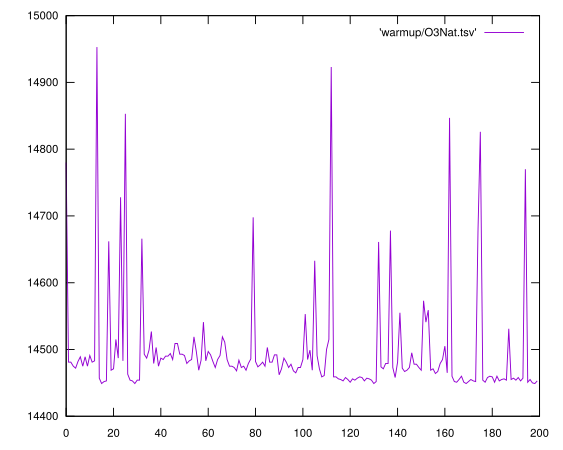
\includegraphics[scale=0.45]{resources/L1/warmup/O3Nat.png}
    \caption{Résultat du warmup avec option \texttt{O3 march=native} du compilateur \textbf{GCC\textsuperscript \textcopyleft  }}
  \end{figure}

  Le résultat obtenu ici est totalement instable, on ne peut pas identifier de stabilisation, donc opérer des warmups ne semble pas avoir de grand intérêt.
  \newpage
\subparagraph{ \texttt{Optimisation Ofast}}
Nous trouvons ce résultat pour L1 :
\begin{figure}[ht!]
  \centering
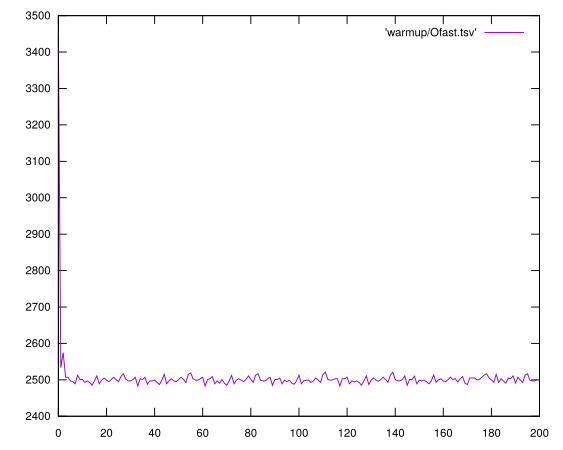
\includegraphics[scale=0.45]{resources/L1/warmup/Ofast.png}
  \caption{Résultat du warmup avec option \texttt{Ofast} du compilateur \textbf{GCC\textsuperscript \textcopyleft  }}
\end{figure}

On observe, comme pour O3, un très court régime transitoire (inférieur à 5 cycles). Un premier warmup de 20 itérations est retenu.

\newpage
\paragraph{Compilateur \texttt{ICC\textsuperscript \textcopyright}}
    \subparagraph{ \texttt{Optimisation O2}}
  Nous trouvons ce résultat pour L1 :
  \begin{figure}[ht!]
    \centering
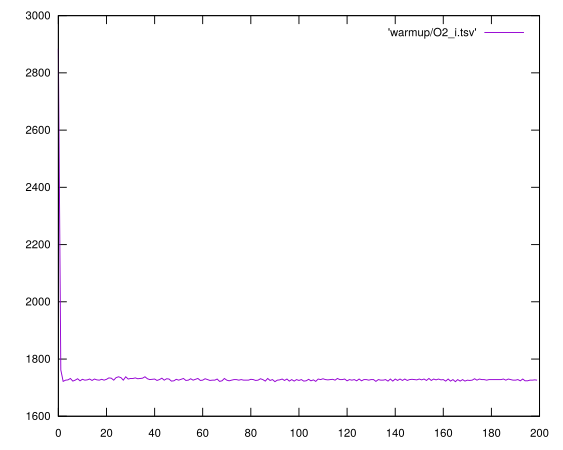
\includegraphics[scale=0.45]{resources/L1/warmup/O2_i.png}
    \caption{Résultat du warmup avec option \texttt{O2} du compilateur \textbf{ICC}}

	Très court régime transitoire, on conserve le nombre de 20 warmups.
  \end{figure}
  \newpage
\subparagraph{ \texttt{Optimisation O3}}
Nous trouvons ce résultat pour L1 :
\begin{figure}[ht!]
  \centering
  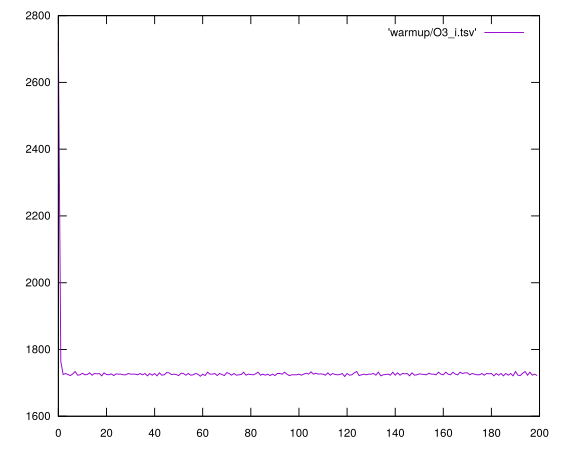
\includegraphics[scale=0.45]{resources/L1/warmup/O3_i.png}
  \caption{Résultat du warmup avec option \texttt{O3} du compilateur \textbf{ICC}}
\end{figure}

Très court régime transitoire, on conserve le nombre de 20 warmups.
\newpage
\subparagraph{ \texttt{Optimisation O3 xHost}}
Nous trouvons ce résultat pour L1 :
  \begin{figure}[ht!]
    \centering
    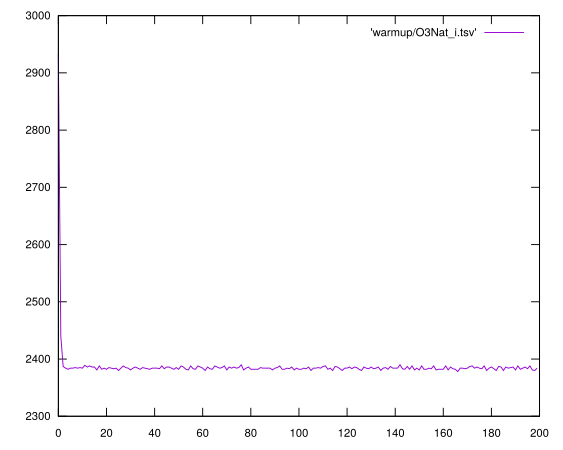
\includegraphics[scale=0.45]{resources/L1/warmup/O3Nat_i.png}
    \caption{Résultat du warmup avec option \texttt{O3 xHost} du compilateur \textbf{ICC}}
  \end{figure}

  Très court régime transitoire, on conserve le nombre de 20 warmups.
  \newpage
\subparagraph{ \texttt{Optimisation Ofast}}
Nous trouvons ce résultat pour L1 :
  \begin{figure}[ht!]
    \centering
    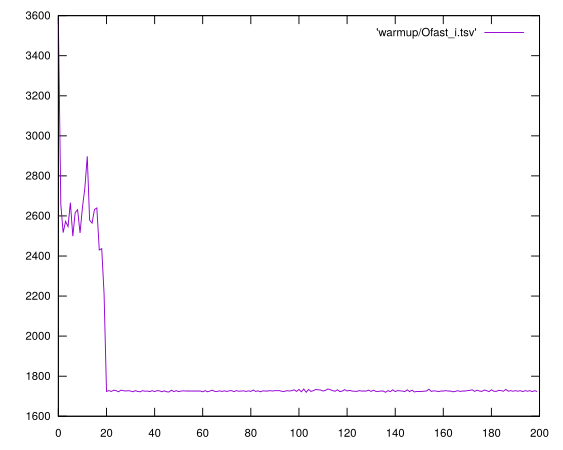
\includegraphics[scale=0.45]{resources/L1/warmup/Ofast_i.png}
    \caption{Résultat du warmup avec option \texttt{Ofast} du compilateur \textbf{ICC}}
  \end{figure}

	Ici, le résultat est différent des cas prédédents : on observe que pendant les 20 premiers warmups on est en régime transitoire et qu'on se stabilise au delà. On prendra donc également 20 warmups.

	Rétrospectivement, étant donné le nombre très faible de warmups nécessaires à chaque configuration d'optimisation (3 ou 20 ne change pas grand chose, on reste dans le même ordre de grandeur), et par souci de simplicité, nous avons arbitrairement fixé à 20 le nombre de warmups pour toutes les options, au regard de celle étudiée dernièrement et en nécessitant plus que les autres.

    \subsubsection{L2 : taille 170, L3 : taille 1000, RAM : taille 20000}
    Les résultats obtenus sont très similaires, on considèrera donc pour chaque optimisation, indépendamment de la taille des données traitées par le noyau, que 20 warmups sont nécessaires à la première méta-répétition, puis on abaissera à 3 warmups pour les méta-répétions suivantes, car la machine est "chaude".
\newpage
\section{Résultats et interprétations}
    \subsection{Compilateur GCC\textsuperscript \textcopyleft  }
      \subsubsection{ \texttt{ Option O2 } }
          \paragraph{Assembleur}
            \begin{tcolorbox}
              \begin{verbatim}
    bcb:	75 f3                	jne    bc0 <baseline+0x30>
    bcd:	83 c1 01             	add    $0x1,%ecx
    bd0:	4c 01 c6             	add    %r8,%rsi
    bd3:	39 cf                	cmp    %ecx,%edi
    bd5:	75 d9                	jne    bb0 <baseline+0x20>
            \end{verbatim}
          \end{tcolorbox}
          \paragraph{MAQAO}
            \begin{tcolorbox}
              \begin{verbatim}
    Vectorization
    -------------
    Your loop is NOT VECTORIZED and could benefit from vectorization.
    By vectorizing your loop, you can lower the cost of an iteration
    from 4.00 to 1.00 cycles (4.00x speedup).
    Since your execution units are vector units,
    only a vectorized loop can use their full power.
            \end{verbatim}
          \end{tcolorbox}
      \subsubsection{ \texttt{ Option O3 }  }
      \paragraph{Assembleur}
        \begin{tcolorbox}
          \begin{verbatim}
bcb:	75 f3                	jne    bc0 <baseline+0x30>
bcd:	83 c1 01             	add    $0x1,%ecx
bd0:	4c 01 c6             	add    %r8,%rsi
bd3:	39 cf                	cmp    %ecx,%edi
bd5:	75 d9                	jne    bb0 <baseline+0x20>
        \end{verbatim}
      \end{tcolorbox}
      \paragraph{MAQAO}
        \begin{tcolorbox}
          \begin{verbatim}
Vectorization
-------------
Your loop is NOT VECTORIZED and could benefit from vectorization.
By vectorizing your loop, you can lower the cost of an iteration
from 4.00 to 1.00 cycles (4.00x speedup).
Since your execution units are vector units,
only a vectorized loop can use their full power.
        \end{verbatim}
      \end{tcolorbox}
      \subsubsection{ \texttt{ Option O3Nat} }
      \paragraph{Assembleur}
        \begin{tcolorbox}
          \begin{verbatim}
bcb:	75 f3                	jne    bc0 <baseline+0x30>
bcd:	83 c1 01             	add    $0x1,%ecx
bd0:	4c 01 c6             	add    %r8,%rsi
bd3:	39 cf                	cmp    %ecx,%edi
bd5:	75 d9                	jne    bb0 <baseline+0x20>
        \end{verbatim}
      \end{tcolorbox}
      \paragraph{MAQAO}
        \begin{tcolorbox}
          \begin{verbatim}
Vectorization
-------------
Your loop is NOT VECTORIZED and could benefit from
vectorization. By vectorizing your loop, you can lower
the cost of an iteration from 4.00 to 1.00 cycles
(4.00x speedup). Since your execution units are vector
units, only a vectorized loop can use their full power.
        \end{verbatim}
      \end{tcolorbox}
      \subsubsection{ \texttt{ Option Ofast } }
      \paragraph{Assembleur}
        \begin{tcolorbox}
          \begin{verbatim}
bc9:	e9 f0 00 00 00       	jmpq   cbe <baseline+0x12e>
bce:	66 90                	xchg   %ax,%ax
bd0:	89 f8                	mov    %edi,%eax
bd2:	c5 fb 58 02          	vaddsd (%rdx),%xmm0,%xmm0
bd6:	83 f8 01             	cmp    $0x1,%eax
bd9:	0f 84 51 01 00 00    	je     d30 <baseline+0x1a0>
        \end{verbatim}
      \end{tcolorbox}
      \paragraph{MAQAO}
        \begin{tcolorbox}
          \begin{verbatim}
Vectorization status
--------------------
Your loop is fully vectorized (all SSE/AVX instructions
are used in vector version (process two or more data elements
in vector registers), using full register length).
        \end{verbatim}
      \end{tcolorbox}
	      \paragraph{Justification}
        \subparagraph{\texttt{Ofast}}
	      Grâce à \texttt{ffast-math} le compilateur ignore les normes et la sécurité, en effet ce flag
        (qui est pratiquement le seul rajouté par le flag \texttt{Ofast} à \texttt{O3}) active les flags
        \texttt{ fno-math-errno, -funsafe-math-optimizations, -fno-trapping-math, -ffinite-math-only, -fno-rounding-math, -fno-signaling-nans}.
        Donc c'est pour cela qu'on arrive à vectorizer notre boucle.
        \subparagraph{\texttt{funroll-loops}}
        Nous remarquons que le code assembleur est différent mais la vectorisation ne change pas, puisque la boucle
        est déjà complètement vectorisé par Ofast
	      \paragraph{Optimisation \texttt{funroll-loops}}
        Le résultat que nous trouvons est :
        \begin{figure}[ht!]
          \centering
          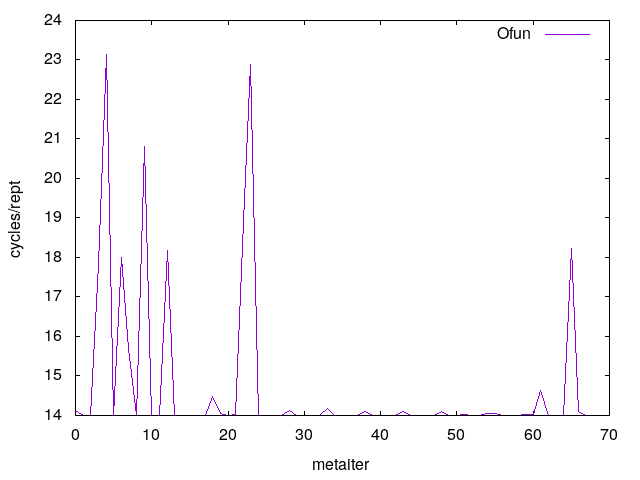
\includegraphics[scale=0.45]{resources/L1/metarep/Ofun.png}
          \caption{Résultat des métarépétitions avec option \texttt{funroll-loops} du compilateur \textbf{GCC\textsuperscript \textcopyleft  }}
        \end{figure}
        \subparagraph{Assembleur}\mbox{} \\
          \begin{tcolorbox}
            \begin{verbatim}
  1322:	0f 86 14 01 00 00    	jbe    143c <baseline+0x1fc>
  1328:	4f 8d 34 f1          	lea    (%r9,%r14,8),%r14
  132c:	45 8d 78 ff          	lea    -0x1(%r8),%r15d
  1330:	41 b9 01 00 00 00    	mov    $0x1,%r9d
  1336:	49 01 f6             	add    %rsi,%r14
  1339:	41 83 e7 07          	and    $0x7,%r15d
  133d:	c4 c1 7d 28 0e       	vmovapd (%r14),%ymm1
  1342:	49 8d 46 20          	lea    0x20(%r14),%rax
  1346:	41 83 f8 01          	cmp    $0x1,%r8d
  134a:	0f 86 d0 00 00 00    	jbe    1420 <baseline+0x1e0>
          \end{verbatim}
        \end{tcolorbox}
        \subparagraph{MAQAO}\mbox{} \\
          \begin{tcolorbox}
            \begin{verbatim}
  Vectorization status
  --------------------
  Your loop is fully vectorized (all SSE/AVX instructions
  are used in vector version (process two or more data elements
  in vector registers), using full register length).
          \end{verbatim}
        \end{tcolorbox}
      \newpage
      \subsection{Compilateur ICC}
      \subsubsection{ \texttt{ Option O2 } }
      \paragraph{Assembleur}
        \begin{tcolorbox}
          \begin{verbatim}
400e39:	72 f2                	jb     400e2d <baseline+0x5d>
400e3b:	49 63 c0             	movslq %r8d,%rax
400e3e:	4d 8d 14 d1          	lea    (%r9,%rdx,8),%r10
400e42:	48 83 c2 08          	add    $0x8,%rdx
400e46:	66 41 0f 58 1a       	addpd  (%r10),%xmm3
400e4b:	66 41 0f 58 52 10    	addpd  0x10(%r10),%xmm2
400e51:	66 41 0f 58 4a 20    	addpd  0x20(%r10),%xmm1
400e57:	66 41 0f 58 42 30    	addpd  0x30(%r10),%xmm0
400e5d:	49 83 c2 40          	add    $0x40,%r10
400e61:	48 3b d0             	cmp    %rax,%rdx
400e64:	72 dc                	jb     400e42 <baseline+0x72>
        \end{verbatim}
      \end{tcolorbox}
      \paragraph{MAQAO}
        \begin{tcolorbox}
          \begin{verbatim}
Vectorization
-------------
Your loop is PARTIALLY VECTORIZED and could benefit from
full vectorization. By fully vectorizing your loop, you can lower
the cost of an iteration from 4.00 to 2.00 cycles (2.00x speedup).
Since your execution units are vector units,
only a fully vectorized loop can use their full power.
        \end{verbatim}
      \end{tcolorbox}
      \subsubsection{ \texttt{ Option O3 }  }
      \paragraph{Assembleur}
        \begin{tcolorbox}
          \begin{verbatim}
400e39:	72 f2                	jb     400e2d <baseline+0x5d>
400e3b:	49 63 c0             	movslq %r8d,%rax
400e3e:	4d 8d 14 d1          	lea    (%r9,%rdx,8),%r10
400e42:	48 83 c2 08          	add    $0x8,%rdx
400e46:	66 41 0f 58 1a       	addpd  (%r10),%xmm3
400e4b:	66 41 0f 58 52 10    	addpd  0x10(%r10),%xmm2
400e51:	66 41 0f 58 4a 20    	addpd  0x20(%r10),%xmm1
400e57:	66 41 0f 58 42 30    	addpd  0x30(%r10),%xmm0
400e5d:	49 83 c2 40          	add    $0x40,%r10
400e61:	48 3b d0             	cmp    %rax,%rdx
400e64:	72 dc                	jb     400e42 <baseline+0x72>
        \end{verbatim}
      \end{tcolorbox}
      \paragraph{MAQAO}
        \begin{tcolorbox}
          \begin{verbatim}
Vectorization
-------------
Your loop is PARTIALLY VECTORIZED and could benefit from
full vectorization. By fully vectorizing your loop, you can lower
the cost of an iteration from 4.00 to 2.00 cycles (2.00x speedup).
Since your execution units are vector units,
only a fully vectorized loop can use their full power.
        \end{verbatim}
      \end{tcolorbox}
      \subsubsection{ \texttt{ Option O3Nat} }
      \paragraph{Assembleur}
        \begin{tcolorbox}
          \begin{verbatim}
400ea1:	72 f3                	jb     400e96 <baseline+0x76>
400ea3:	48 63 d0             	movslq %eax,%rdx
400ea6:	c5 e5 58 1c ce       	vaddpd (%rsi,%rcx,8),%ymm3,%ymm3
400eab:	c5 ed 58 54 ce 20    	vaddpd 0x20(%rsi,%rcx,8),%ymm2,%ymm2
400eb1:	c5 f5 58 4c ce 40    	vaddpd 0x40(%rsi,%rcx,8),%ymm1,%ymm1
400eb7:	c5 fd 58 44 ce 60    	vaddpd 0x60(%rsi,%rcx,8),%ymm0,%ymm0
400ebd:	48 83 c1 10          	add    $0x10,%rcx
400ec1:	48 3b ca             	cmp    %rdx,%rcx
400ec4:	72 e0                	jb     400ea6 <baseline+0x86>
        \end{verbatim}
      \end{tcolorbox}
      \paragraph{MAQAO}
        \begin{tcolorbox}
          \begin{verbatim}
Vectorization status
--------------------
Your loop is fully vectorized (all SSE/AVX instructions
are used in vector version (process two or more data elements
in vector registers), using full register length).
        \end{verbatim}
      \end{tcolorbox}
      \subsubsection{ \texttt{ Option Ofast } }
        \paragraph{Assembleur}
          \begin{tcolorbox}
            \begin{verbatim}
  400e39:	72 f2                	jb     400e2d <baseline+0x5d>
  400e3b:	49 63 c0             	movslq %r8d,%rax
  400e3e:	4d 8d 14 d1          	lea    (%r9,%rdx,8),%r10
  400e42:	48 83 c2 08          	add    $0x8,%rdx
  400e46:	66 41 0f 58 1a       	addpd  (%r10),%xmm3
  400e4b:	66 41 0f 58 52 10    	addpd  0x10(%r10),%xmm2
  400e51:	66 41 0f 58 4a 20    	addpd  0x20(%r10),%xmm1
  400e57:	66 41 0f 58 42 30    	addpd  0x30(%r10),%xmm0
  400e5d:	49 83 c2 40          	add    $0x40,%r10
  400e61:	48 3b d0             	cmp    %rax,%rdx
  400e64:	72 dc                	jb     400e42 <baseline+0x72>
          \end{verbatim}
        \end{tcolorbox}
          Ofast inclus moins de vectorisation que \texttt{O3 -xHost} donc c'est l'option xHost
          qui nous permet de passer de addpd vers vaddpd.
        \paragraph{MAQAO}
        \begin{tcolorbox}
          \begin{verbatim}
Vectorization
-------------
Your loop is PARTIALLY VECTORIZED and could benefit from full
vectorization. By fully vectorizing your loop, you can lower
the cost of an iteration from 4.00 to 2.00 cycles (2.00x speedup).
Since your execution units are vector units,
only a fully vectorized loop can use their full power.
        \end{verbatim}
      \end{tcolorbox}
      \subsubsection{\texttt{ Option funroll-loops}}
        Le résultat que nous trouvons est :
        \begin{figure}[ht!]
          \centering
          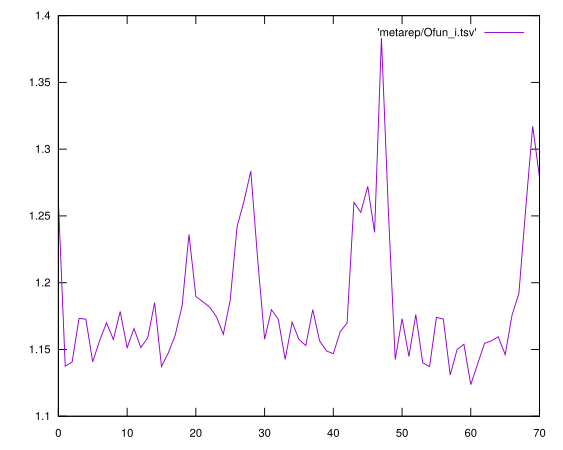
\includegraphics[scale=0.45]{resources/L1/metarep/Ofun_i.png}
          \caption{Résultat des métarépétitions avec option \texttt{funroll-loops} du compilateur \textbf{ICC}}
        \end{figure}
        \paragraph{Assembleur}
          \begin{tcolorbox}
            \begin{verbatim}
  400ea1:	72 f3                	jb     400e96 <baseline+0x76>
  400ea3:	48 63 d0             	movslq %eax,%rdx
  400ea6:	c5 e5 58 1c ce       	vaddpd (%rsi,%rcx,8),%ymm3,%ymm3
  400eab:	c5 ed 58 54 ce 20    	vaddpd 0x20(%rsi,%rcx,8),%ymm2,%ymm2
  400eb1:	c5 f5 58 4c ce 40    	vaddpd 0x40(%rsi,%rcx,8),%ymm1,%ymm1
  400eb7:	c5 fd 58 44 ce 60    	vaddpd 0x60(%rsi,%rcx,8),%ymm0,%ymm0
  400ebd:	48 83 c1 10          	add    $0x10,%rcx
  400ec1:	48 3b ca             	cmp    %rdx,%rcx
  400ec4:	72 e0                	jb     400ea6 <baseline+0x86>
          \end{verbatim}
        \end{tcolorbox}
        Nous remarquons que contrairement à \texttt{Ofast} l'option \texttt{funroll-loops} utilise \textbf{vaddpd}
        au lieu de \textbf{addpd}, et le résultat de \textit{MAQAO} montre que notre boucle est bel et bien vectorisé
       \paragraph{MAQAO}
        \begin{tcolorbox}
          \begin{verbatim}
Vectorization status
--------------------
Your loop is fully vectorized (all SSE/AVX instructions
are used in vector version (process two or more data elements
in vector registers), using full register length).
        \end{verbatim}
      \end{tcolorbox}
        Les médianes des différents temps d'exécution :\\
        \begin{tabular}{|c| c | c |}
          \hline
        \multirow{5}{*}{GCC \textsuperscript \textcopyleft} & \texttt{-O2} & $3.964161$  \\ \cline{2-3}
              & \texttt{-O3}                                  & $3.964172$  \\ \cline{2-3}
           & \texttt{-O3 -march=native}                    & $3.964278$  \\ \cline{2-3}
              & \texttt{-Ofast -march=native}                 & $0.824717$  \\ \cline{2-3}
              & \texttt{-Ofast -march=native -funroll-loops}  & $1.036789$  \\ \hline
      \multirow{5}{*}{ICC \textsuperscript \textcopyright}   & \texttt{-O2} & $0.476589$  \\ \cline{2-3}
              & \texttt{-O3}                                  & $0.476239$  \\ \cline{2-3}
           & \texttt{-O3 -xHost}                           & $0.645322$  \\ \cline{2-3}
              & \texttt{-Ofast -xHost}                        & $0.476617$  \\ \cline{2-3}
              & \texttt{-Ofast -xHost -funroll-loops}         & $0.645228$  \\
        \hline
        \end{tabular}
\end{document}
